% !TEX encoding = UTF-8 Unicode
\documentclass[10pt,twocolumn,letterpaper]{article}

\usepackage[utf8]{inputenc}
\usepackage[T1]{fontenc}
\usepackage{textcomp,gensymb}
\usepackage{ae,aecompl}

\usepackage[english]{babel}
\usepackage[none]{hyphenat}

\usepackage{cvpr}
\usepackage{times}
\usepackage{epsfig,graphicx}
\usepackage{amsmath,amssymb}

\usepackage{enumitem}
\setlist{nosep}

\usepackage{multirow}

% Include other packages here, before hyperref.

% If you comment hyperref and then uncomment it, you should delete
% egpaper.aux before re-running latex.  (Or just hit 'q' on the first latex
% run, let it finish, and you should be clear).
\usepackage[breaklinks=true,bookmarks=false,hidelinks=true]{hyperref}

\cvprfinalcopy

%\def\cvprPaperID{****} % *** Enter the CVPR Paper ID here
%\def\httilde{\mbox{\tt\raisebox{-.5ex}{\symbol{126}}}}

\setcounter{page}{1}
\begin{document}

\title{XXXXXXXXXXXXXXXXXXXXXXXXXXXXXXXXXXX}

\author{Nicolò Bertozzi\\
S276406\\
{\tt\small nicolo.bertozzi@studenti.polito.it}
\and
Francesco Bianco Morghet\\
S277910\\
{\tt\small s277910@studenti.polito.it}
}

\maketitle
%\thispagestyle{empty}


\begin{abstract}
\end{abstract}


\section{Introduction}

One of the main challenges in the field of Computer Vision and Artificial Intelligence lies in the recognition of the actions included inside a video. Until now, the research has been concentrated on the data provided by specific kinds of cameras, used in particular ares and in particular places, which capture the alternating of the everyday life from an external narrator point of view, i.e in third person.

A lot of areas are interested in a classification based on first person videos. Among them, the robotic applications could be surely cited, starting from the definition of the androids’ intelligence like iCub\textsuperscript{\textcopyright} to the autonomous driving, together with the surveillance, the composition of the people’s behavioral profile, in order to predict and then to prevent potential offenses, the analysis of the users’ content information to allow a tracking of their preferences loyalizing their experience inside the service etc.

The datasets which contains this information, until now, are very small but, in the future with the growing increase of the sale of wearable devices, with the undeterred increment of the ease to have at our disposal a camera and with the exponential growth of the number of photos and videos taken every day in all over the world, this limit could be easily surpassed. 

In addition the first person images present further difficulties than the one in third person. First of all, it is very frequent to observe inside this videos limbs of him who is capturing the action. So this features has to be used in order to promote the action recognition and not to disadvantage the task. Then it is very probable that the camera which is taking the video is mounted on the head of the subject who is performing the operation and if so also the perspective change basing on what the cameraman is watching in that moment.

Dependently on the context, the video classification could be more precise or less precise. A general purpose recognition can be summarized by a simple verb, which defines without accuracy the action in progress. Instead a more careful recognition is composed by a verb plus a noun. In fact the difference between the task \emph{open} and \emph{open a door} and still \emph{open a jar} is completely different.

\section{Related works}

In this section we introduce some of the recent approaches used to process first person videos along with some of the employed preprocessing techniques.

\subsection{Optical flow and warped optical flow}

In order to encode motion of objects and isolate it from their appearance, optical flow is often employed in many machine learning approaches.

The main assumption of the optical flow extraction procedure is that, between two still frames, objects have moved by a small amount, if any, and their brightness has not changed. This is not always true: for instance, an object could fall inside the shadow cast by another object, therefore altering their brightness. Formally, by writing the brightness $I$ as function of space $x,y$ and time $t$, the following equation can be expressed:
${I(x,y,t) = I(x + \Delta x, y + \Delta y, t + \Delta t)}$. By rewriting the right member as its Taylor expansion up to its first term, the following holds: $\nabla I \cdot \vec{V} = -I_t$. In this single equation, both the $x$ component and the $y$ component of velocity $V$ are unknown. This is described as the aperture problem, and so, to actually compute the optical flow, further constraints are put in place.

A main issue with optical flow is that camera motion highly influences the process, thus adding unnecessary noise to the computed results. So, in order to subtract camera motion, in \cite{wang2013trajectiories} the warped optical flow is introduced. It consists in inferring the global background motion by estimating the homography matrix and then subtracting the camera motion from the computed optical flow. This second procedure is particularly useful for removing noisy movements in the first person point of view videos, as in the case of an action cam mounted on a shoulder of a person.

\subsection{Two-stream approach}

The first person action recognition task has been tackled by several works in recent years, and various solutions involving deep learning algorithms have been proposed.

In most works, a convolutional neural network, such as a ResNet-34, is used to extract feature embeddings from RGB images; then, a Convolutional Long Short-Term Memory (ConvLSTM) is used to model the temporal dependencies between the feature maps extracted by the convolutional segment and the spatial correlations inside each of those; finally, a linear classifier on the features extracted by the ConvLSTM is used to classify the portrayed action.

However, the aforementioned model focuses on the appearances of each single frame, but it fails to take into account the motion happening in those frames in a effectively manner. To tackle this problem, a separate convolutional neural network can be trained on optical flows images.

Then, on top of these two trained networks, a linear classifier is used to determine the class label of the given sample: while the classifier is trained on the output features of the two networks, the two networks are fine tuned on the weights obtained in a preceding set of training stages.

The main disadvantage of this two stream approach is that motion information and appearance information are decoupled, and so, since they are treated in two separate networks, any correlations among the two are not taken into account.

There exist however an attempts to go beyond the two streams approach and to deal with both appearance and motion in a single network by using an auxiliary task, as in the case of \cite{planamente2020joint} where a motion segmentation task is deployed.

\subsection{Attention model}
\label{par:AttentionModel}
One milestone for the development of a working solution for recognising the involved action is the acknowledgement of the important role played by the motion of the hands and the appearance of the objects in the scene. So, focusing the attention on the most important region of a frame of a video, while at the same time discarding irrelevant information, can be a key component for getting a great performance gain in terms of accuracy. For this reason, in \cite{Ego-RNN} an attention mechanism is employed in the ResNet backbone in order to extract features with spatial attention.

To extract features with spatial attention $f_{SA}$, \textit{class activation maps} (CAMs) are employed:
\begin{enumerate}
	\item The $l$ output feature maps of the very last convolutional layer of the backbone are forwarded to an average pool that reduces each feature map size to a 1x1 block, then those reduced feature maps are forwarded to a fully connected layer;
	\item The CAM for class $c$ is obtained, for each spatial location $i$, by dot multiplying the values of the $l$ feature maps at location $i$ and the weights of the neuron of the fully connected layer of class $c$, i.e. ${\text{CAM}_c(i) = \sum_l w_l^c f_l(i)}$. 
	\item The features with spatial attention $f_{SA}$ are obtained by performing the Hadamard product between the output feature maps of the very last convolutional layer of the backbone and the output of the softmax operation applied to the CAM of the class with the highest probability.
\end{enumerate}

The limit of the attention mechanism is that it almost completely discards any motion information but it only focuses on the appearance of each single frame. So, despite the deployment of the attention mechanism, in \cite{planamente2020joint} in order to reach state of the art performances, a separate convolutional neural network is trained on stacked warp flow images, and then, a linear classifier is put on top of the output features of the two networks.

\subsection{Motion segmentation task}
The main idea behind this procedure is the addition of an auxiliary task: given an architecture where first a convolutional neural network extracts feature embeddings from RGB frames and then a ConvLSTM models temporal and infra-spatial correlations of such features, a second task is added to the output of the convolutional neural network with the intention of helping this shared backbone to extract more meaningful features and taking motion into account as well.

In \cite{planamente2020joint}, a motion segmentation task is proposed. To do so, an \textit{improved dense trajectory} (IDT) is associated to each frame; basically, an IDT is a binary map that compensates for camera motion and that, for each pixel, states whether a moving keypoint is present or not. This motion map is used as a ground truth for a motion segmentation task: the output feature maps of the last convolutional layer of the shared backbone are forwarded to a second branch where they are first processed by a convolutional layer and then forwarded to a fully connected layer. This auxiliary task aims to minimise the pixel-by-pixel cross entropy loss between the predicted motion map and the ground truth. Both auxiliary task and main task tasks are trained together, because the role of the auxiliary task is to help the shared backbone to extract better features, in the sense that they are able to into account motion as well: for this reason, the losses of the auxiliary task and the main task are summed together during training.


\section{Proposed method}
Our method is based on the fact that the employment of optical flow has been proved to be effective to capture and encode motion cues from moving objects. In this work, the warp flow is used since, as it has been introduced in the paragraphs above, it allows for the compensation of camera movements, which is a great factor to take into account in first person videos.

Our proposed method draws its inspiration from \cite{carlucci2017de2}, where a convolutional neural network is used to colorise depth images. Our method extracts RGB frames from warp flow frames: by leveraging a pre-existing RGB network which features a ResNet-34 backbone already trained on ImageNet, our method aims to replicate the results obtained by this architecture achieved on standard RGB frames.

So, the employed method can be decomposed into two macro steps, which are briefly presented here and will be discussed in more details in the following paragraphs:
\begin{enumerate}
	\item A convolutional neural network, which will be referred to as WFCNet from this point on, is trained so that a mapping between warp flow frames and generated RGB frames is learnt; 
	\item Using WFCNet for inferring RGB frames from warp flow frames, a deep neural network consisting in a convolutional backbone, a ConvLSTM, an average pooling layer and a final fully connected layer is trained in a multi stage manner; we also propose a two stream variant, which consists in a shared backbone, fed with both colorised warp flow frames and original RGB frames, and whose output features are fed to two ConvLSTMs.
\end{enumerate}

\subsection{WFCNet}

\begin{figure*}[t]
	\begin{center}
		\includegraphics[width=\textwidth]{schemi/WFCNet.img.pdf}		
	\end{center}
	\caption{WFCNet module representation along with the whole architecture used in the training phase}
	\label{fig:WFCNet}
\end{figure*}

WFCNet is a ResNet like network: it makes use of residual blocks which introduce additional direct connections from input to output that skip convolutional layers. This procedure enables a better gradient flow in the backward propagation step and prevents the gradient vanishing problem that limits the deepness of neural networks.

WFCNet is made of basic blocks; each block consists in: two convolutional layers with kernel size of 3, stride of 1 and padding of 1; one ReLu between them; batch normalisation at the output of each convolutional layer; a direct connection from input to output, which is obtained by summing the input of the block to the output of the second convolution.
As suggested by the work presented in \cite{springenberg2014striving}, the downsampling of the residual input is done by using a convolutional filter instead of a simple average pooling: in this way, an embedding can be learnt leading to better downsampled feature maps, while at the same time the advantages of the residual block are preserved.
The upsampling of the residual input is performed instead by applying a nearest neighbour resizing followed by a convolution filter with a stride 1 and kernel size of 1.

These basic blocks are grouped together in blocks that we can call macro blocks. It should be noted that the downsampling or upsampling are performed only by the first convolutional layer of each macro block. The downsampling is the result of the adoption of a convolution with a stride of 2, kernel size of 3 and padding of 1; on the other hand, the upsampling is performed using a nearest neighbour resizing followed by a convolutional filter with a stride 1, kernel size of 3 and padding of 1 on every side. 

This structure with gradual downsampling followed by a gradual upsampling allows for the extraction of RGB images with semantic segmentation for hands and objects involved in the action, while at the same time all the other still objects are discarded and melted with the background. In this work, the transposed convolution for upsampling is not employed because its introduction resulted in repeating patterns in the output RGB frames that would not disappear even after many epochs of training: the employment of nearest neighbour for upsampling instead leads to better segmented images, which in turn leads to better overall results.

Finally, the output RGB frames of WFCNet are normalised: first the Sigmoid function is applied to every output value in order to get values in the $[-1; +1]$ range; then, every channel of each pixel is normalised on the means and standard deviations of ImageNet, which are \texttt{mean=[0.485, 0.456, 0.406]}, \texttt{std=[0.229, 0.224, 0.225]}. The introduction of this block improves the performances of the model and its stability at the beginning of the training because, in the overall training procedure of this network, a ResNet-34 pre-trained on ImageNet is employed. Also, since WFCNet is later employed to colorise frames which are then fed to an RGB network whose backbone is pre-trained on ImageNet, it is important that those generated images are normalised in the correct manner in order to achieve optimal results. By explicitly introducing this block, we can be sure that the generated images meet this requirement.

\begin{table}
	\begin{tabular}{l|lp{40mm}}
	Conv 0 & CONV & 2x7x7x8, s=2, p=3 \\
	
	\hline
	\multirow{6}{*}{\shortstack{Conv 1\\(x2)}} & CONV & 8x3x3x8, s=1, p=1 \newline (s=2 for 1st block) \\
	& BN & \\
	& RELU & \\
	& CONV & 8x3x3x8, s=1, p=1 \\
	& BN & \\
	& RES & \\
	
	\hline
	\multirow{6}{*}{\shortstack{Conv 2\\(x3)}} & CONV & 16x3x3x16, s=1, p=1 \newline (8x3x3x16, s=2 for 1st block) \\
	& BN & \\
	& RELU & \\
	& CONV & 16x3x3x16, s=1, p=1 \\
	& BN & \\
	& RES & \\
	
	\hline
	& UPSAMPLE & factor=2 \\
	& CONV & 16x1x1x16, s=1, p=0 \\
	
	\hline
	\multirow{6}{*}{\shortstack{Deconv 1\\(x3)}} & CONV & 16x3x3x16, s=1, p=1 \\
	& BN & \\
	& RELU & \\
	& CONV & 16x3x3x16, s=1, p=1 \\
	& BN & \\
	& RES & \\
	
	\hline
	& UPSAMPLE & factor=2 \\
	& CONV & 16x1x1x16, s=1, p=0 \\
	
	\hline
	\multirow{6}{*}{\shortstack{Deconv 2\\(x2)}} & CONV & 8x3x3x8, s=1, p=1 \newline (16x3x3x8, for 1st block) \\
	& BN & \\
	& RELU & \\
	& CONV & 8x3x3x8, s=1, p=1 \\
	& BN & \\
	& RES & \\
	
	\hline
	\multirow{2}{*}{  Out} & CONV & 8x1x1x3, s=1, p=1 \\
	& NORM & \\
	
\end{tabular}
	\vspace{5mm}
	\label{tab:wfcnet}
	\caption{WFCNet detailed structure}
\end{table}

\subsection{Training WFCNet}
\label{par:TrainingWFCNet}

The aim of the WFCNet block is to learn a mapping from input warp flow frames to output RGB frames.

We propose two variants for WFCNet, which differ in the kind of input they accept:
\begin{enumerate}
	\item One single warp flow frame, consisting in two channel, i.e. the x-axis displacement and the y-axis displacement;
	\item A stack of five consecutive warp flow frames, which account to a total number of 10 channels.
\end{enumerate}

In order to train WFCNet, a ResNet-34, followed by an average pooling and a fully connected layer, are employed. The complete architecture is represented in figure \ref{fig:WFCNet}: the input frame is colorised by WFCNet; then the resulting RGB image is fed to the ResNet-34; finally, the output features of the ResNet-34 are forwarded to the classification block, which consists in an average pooling (which reduces the feature maps from a 512x7x7 volume to a vector of 512 elements) and a fully connected layer.

Each video sample consists in possibly more than one input frame, accounting for different time steps: for this reason, for each sample, multiple input frames are forwarded to the network, multiple RGB images are generated and so multiple output scores are produced by the final fully connected layer. For this reason, the average of the output scores is computed with respect to the time dimension.

We treat this task as a classification problem, where the aim of the whole architecture (consisting in WFCNet, ResNet, and classification block) is to predict the class label of the sample. For this reason, the \textit{Cross Entropy Loss} is employed, which can be expressed as ${L = -\sum_i^N{\log(P(y_i | x_i, w))}}$, where $N$ is the total number of samples, $x_i$ is the input sample, $y_i$ is the true label, and ${P(y_i | x_i, w)}$ is the predicted probability for the true label $y_i$ given the sample $x_i$ and the weights of the network $w$. The normalised probabilities for the different classes are computed using the softmax function: ${P(y_i | x_i, w) = \frac{e^{f_{y_i}}}{\sum_i e^{f_i}}}$.

The whole training procedure consists in two main stages:
\begin{enumerate}
	\item The ResNet-34 is pre-trained on ImageNet and its weights are kept frozen; the weights of WFCNet are randomly initialised using the uniform distribution according to the Kaiming procedure described in \cite{he2015delving}. Only the weights of WFCNet and the weights of the final fully connected layers are trained;
	\item In this second stage, besides fine tuning the weights of WFCNet and the final fully connected layer, also the weights of the very last ``macro block'' of the ResNet-34 are fine tuned: in this way, the performances of the whole architecture are improved.
\end{enumerate}
It should be noted the performances of this architecture are not interesting \textit{per se}, since we are only interested in later reusing the WFCNet block in another network better suited for the action recognition task, i.e. the RGB network. However, we qualitatively observed to be present a positive correlation between high performances of this architecture and high performances of WFCNet in conjunction with the RGB network: so we employ this multi stage training for this particular reason.

\subsection{Single-Stream RGB network}

\begin{figure*}
	\begin{center}
		\includegraphics[width=\textwidth]{schemi/single_stream.img.pdf}		
	\end{center}
	\caption{Single-stream RGB network}
	\label{fig:SingleStream}
\end{figure*}

The single-stream RGB network is closely inspired by the RGB network proposed in \cite{Ego-RNN}, but it performs the action recognition task on warp flow frames.

The structure of the network is represented in figure \ref{fig:SingleStream} and it consists of:
\begin{enumerate}
	\item A WFCNet module, which is pre-trained in a previous stage as described in the paragraph \ref{par:TrainingWFCNet} and it is used to infer the RGB frames starting from warp flow frames;
	\item a ResNet-34 pre-trained on ImageNet;
	\item an attention mechanism, as described in paragraph \ref{par:AttentionModel}, which is used to extract features with spatial attention $f_{SA}$ from the convolutional backbone;
	\item a ConvLSTM which is used to model the temporal and spatial correlations of the extracted feature maps with spatial attention;
	\item an average pooling layer followed by a fully connected layer.
\end{enumerate}

The structure of the ConvLSTM is the same as the one employed in \cite{Ego-RNN}. The main differences from a standard LSTM cell is that a ConvLSTM cell performs convolutional operations in place of matrix multiplications, and that input and state data are represented with 3D tensors so that spatial encoding can also be performed.
Therefore the reasons of using a ConvLSTM are the following ones:
\begin{itemize}
	\item There is the need to perform temporal encoding of the input features;
	\item A simple Recurrent Neural Network consisting of a single state vector suffers from the gradient vanishing problem; an LSTM cell instead performs the necessary operations to attenuate this problem;
	\item ConvLSTM cells have been proved to be effective in encoding spatial and temporal changes simultaneously.
\end{itemize}
The operations performed by the ConvLSTM can be represented by the following equations:
\begin{equation*}
\begin{gathered}
i_t = \sigma(w_x^i * x + w_h^i * h_{t-1} + b_i) \\
f_t = \sigma(w_x^f * x + w_h^f * h_{t-1} + b_f) \\
o_t = \sigma(w_x^o * x + w_h^o * h_{t-1} + b_o)\\
\tilde{c}_t = \tanh(w_x^c * x + w_h^c * h_{t-1} + b_{\tilde{c}}) \\
c_t = \tilde{c}_t \odot i_t + c_{t-1} \odot f_t \\
h_t = o_t \odot \tanh(c_t)
\end{gathered}
\end{equation*}
where $x$ is the input, $\sigma$ is the sigmoid function, $i$, $f$, $o$ and $\tilde{c}_t$ are the four gates, $h$ and $c$ are respectively hidden state and memory state.
The weights of the convolutions are initialised by sampling a normal distribution according to the Xavier procedure.

Being this a classification problem, the \textit{Cross Entropy Loss} is employed, which can be expressed as ${L = -\sum_i^N{\log(P(y_i | x_i, w))}}$, where $N$ is the total number of samples, $x_i$ is the input sample, $y_i$ is the true label, and ${P(y_i | x_i, w)}$ is the predicted probability for the true label $y_i$ given the sample $x_i$ and the weights of the network $w$. The normalised probabilities for the different classes are computed using the softmax function: ${P(y_i | x_i, w) = \frac{e^{f_{y_i}}}{\sum_i e^{f_i}}}$.

During the training phase, the WFCNet block is always used in inference mode; the training is performed in two stages:
\begin{enumerate}
	\item In the first stage, the final fully connected layer and the ConvLSTM cell are trained, while the weights of the rest of the network are kept frozen;
	\item In the second stage, besides fine tuning the final fully connected layer and the ConvLSTM cell, also the last ``macro block'' of the backbone and the hidden fully connected layer used for extracting the CAMs are fine tuned.
\end{enumerate}

\subsection{Two-Stream RGB network}

%\begin{figure*}
%	\begin{center}
%		\includegraphics[width=\textwidth]{schemi/two_stream.img.pdf}		
%	\end{center}
%	\caption{Two-stream RGB network}
%	\label{fig:TwoStream}
%\end{figure*}

We do realise that, in order to perform the action recognition task in the first person point of view, the warp flow by itself may not be sufficient to achieve discrete performances. For this reason, we propose a two-stream network.

\section{Experimental results}

In this section we first introduce the dataset that we used in this work, then we describe the experiments that we performed on it.

\subsection{Dataset}

\begin{figure}
	\begin{center}
		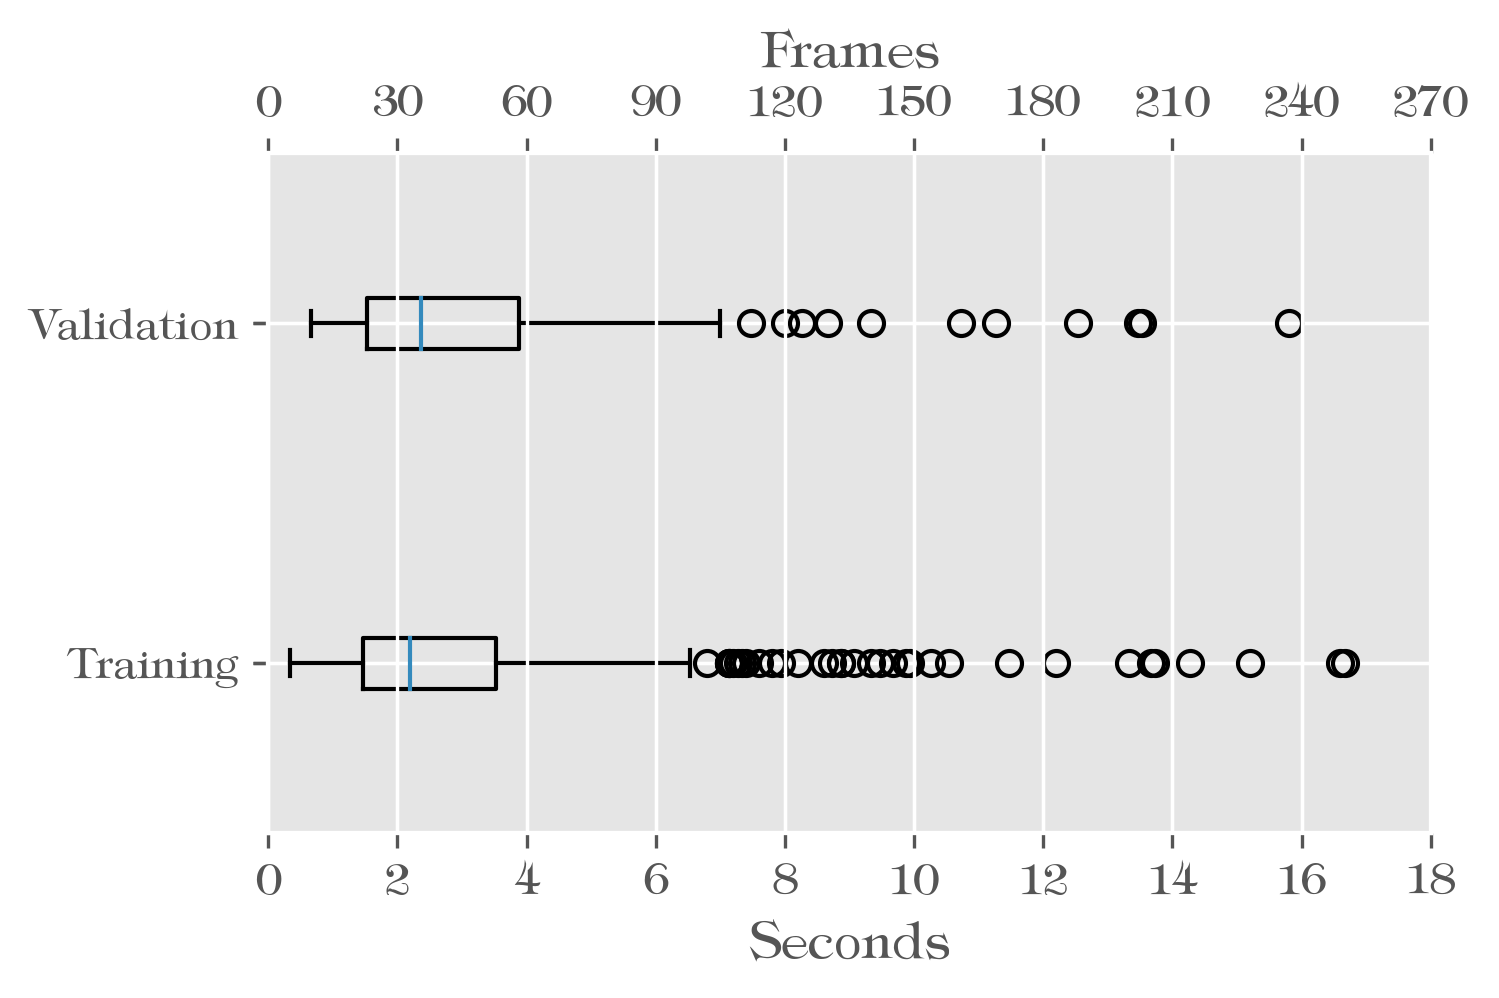
\includegraphics[width=\linewidth]{grafici/GTEA61_boxplot.png}		
	\end{center}
	\caption{GTEA-61 dataset; box-plots of sample lengths. A sample length is considered as outlier (and so represent as circle) if its value is greater than $Q_3 + 1.5(Q_3-Q_1)$, where $Q_i$ are quartiles}
	\label{fig:GTEA61_boxplot}
\end{figure}

The GTEA-61 dataset contains several video clips recorded at 15 fps which portrays 7 common activities performed by 4 different subjects in a first person point of view. The actions are further divided into subcategories consisting in verb+object, such as \textit{open tea}, therefore totalling 61 different labels. In this work, we consider a constant split of the labelled data: specifically we always consider the actions performed by S2 as validation data.

In figure \ref{fig:GTEA61_boxplot}, the distribution of the lengths of the video clips are represented by means of a pair of box-plots: as it can be seen, even though durations greatly vary, at least 75\% of both training and validation data is below 4 seconds. Unless stated otherwise, during our experiments we sample a fixed number of frames uniformly spaced in time. This means that for the great majority of the clips, the time span between two frames is a certain fraction of a second, ranging from less than one-tenth to half a second. However, there are edge cases in which the time elapsed between two frames can be significantly higher or some other cases in which frames are being duplicated, as in the case in which $N = 16$ frames are sample but the clip is less shorter than a second. This may negatively impact the performances of the experimented models.

\subsection{Ego-RNN}

\subsection{Self supervised task}

\section{Conclusions}

{\small
\bibliographystyle{ieee_fullname}
\bibliography{egbib}
}

\end{document}
